\section{Przygotowanie modelu}
% Delete the text and write your Results here:
%------------------------------------

\subsection{DecisionTreeClassifier}
\label{DTC}
\hspace{\parindent}
DecisionTreeClassifier jest algorytmem uczenia maszynowego, który opiera się na drzewach decyzyjnych do problemów klasyfikacji. Jest to jeden z najprostszych i najbardziej intuicyjnych algorytmów uczenia maszynowego.

Drzewo decyzyjne składa się z węzłów i krawędzi, które reprezentują decyzje oparte na wartościach cech. Algorytm uczący DecisionTreeClassifier tworzy drzewo decyzyjne na podstawie dostępnych danych treningowych, które składają się z przykładów oznaczonych etykietami klas.

Algorytm działa następująco:
\begin{enumerate}
    \item Wybór najlepszej cechy, która podzieli zbiór danych na sposób, który najlepiej separuje przykłady klas.
    \item Podział danych na podstawie wartości wybranej cechy, tworzący węzeł decyzyjny.
    \item Powtarzanie kroków 1-2 rekurencyjnie dla każdego nowo utworzonego węzła, aż zostaną spełnione pewne kryteria stopu.
    \item Przypisanie etykiety klasy do liści drzewa na podstawie większościowych etykiet przykładów uczących w danym liściu.
\end{enumerate}

\subsection{RandomForestClassifier}
\label{RFC}
\hspace{\parindent}
RandomForestClassifier jest algorytmem uczenia maszynowego, który opiera się na zasadzie ensemble learning, czyli łączeniu wyników wielu modeli w celu uzyskania lepszej jakości predykcji. Jest oparty na metodzie drzew decyzyjnych.

RandomForestClassifier tworzy wiele drzew decyzyjnych na podstawie losowych podzbiorów danych treningowych. Każde drzewo jest trenowane niezależnie na różnych podzbiorach danych. Podczas prognozowania klasyfikacji każde drzewo decyzyjne w lesie przewiduje wynik, a ostateczna predykcja jest dokonywana na podstawie głosowania większości.

Ważną cechą RandomForestClassifier jest wprowadzenie losowości poprzez losowe wybieranie podzbiorów cech do trenowania każdego drzewa. Dzięki temu zapobiega się overfittingowi (przeuczeniu), gdy model zbytnio dopasowuje się do danych treningowych.

Dodatkowo, podczas trenowania każdego drzewa, stosuje się losowanie ze zwracaniem, co oznacza, że każdy podzbiór danych ma możliwość zawierać duplikaty próbek. Ta technika znana jako bagging (bootstrap aggregating) pomaga zwiększyć różnorodność drzew w lesie i zmniejszyć wariancję modelu.

\subsection{Przygotowanie modelu dla naszego zbioru}
\hspace{\parindent}

Nasze dane podzielimy na zbiór treningowy i testowy w stosunku 1:3, co pozwoli na odpowiednie nauczenie modelu.

Po wytrenowaniu naszego modelu oraz wytestowaniu go otrzymujemy następujące wyniki:
\begin{table}[htbp]
\centering
\caption{Wyniki F1-score dla różnych modeli}
\label{tab:results}
\begin{tabular}{|l|c|c|c|c|}
\hline
\multirow{2}{*}{Model} & \multicolumn{4}{c|}{F1-score} \\
\cline{2-5}
& Motoryzacja & Muzyka & Sport & Rozrywka \\
\hline
DTC & 0.67 & 0.75 & 0.69 & 0.68 \\
\hline
RFC & 0.76 & 0.84 & 0.79 & 0.79 \\
\hline
\end{tabular}

\vspace{10pt}

\begin{tabular}{|l|c|c|c|c|}
\hline
\multirow{2}{*}{Model} & \multicolumn{4}{c|}{F1-score} \\
\cline{2-5}
& WiP & Dokładność & Arytmetyczna & Ważona \\
\hline
DTC & 0.85 & 0.73 & 0.73 & 0.73 \\
\hline
RFC & 0.9 & 0.82 & 0.82 & 0.82 \\
\hline
\end{tabular}
\end{table}

WiP\footnote{Wiadmości i polityka}

F1-score jest miarą oceny jakości klasyfikacji. Jest to średnia harmoniczna precyzji (precision) i czułości (recall) klasyfikatora. Czułość to miara, która mierzy zdolność klasyfikatora do wykrywania rzeczywiście pozytywnych przypadków, podczas gdy precyzja ocenia, ile zidentyfikowanych jako pozytywne przypadków jest faktycznie poprawnych.

Dokładność (accuracy) to miara, która mierzy ogólną skuteczność klasyfikatora poprzez porównanie liczby poprawnie sklasyfikowanych przypadków do całkowitej liczby przypadków. Średnia arytmetyczna (macro avg) to miara dla każdej klasy, niezależnie od rozmiaru klasy. Średnia ważona (weighted avg) to miara dla każdej klasy, z wagami proporcjonalnymi do liczności klas. Ponieważ w zbiorze mamy bardzo zbliżoną liczbę rekordów poszczególnych kategorii, dlatego wyniki w tych polach są w przybliżeniu taki same.

Jak widzimy na tabelce nasze modele najlepiej radzą sobie w przewidywaniu wiadomości i polityki oraz nieco gorzej radzą sobie z muzyką.

Ogólnie również możemy zaobserwować, że model RFC radzi sobie lepiej aż o 9 punktów procentowych niż model DTC, który uzyskuje wynik na poziomie 73\%.

Nasze dane możemy również zaprezentować za pomocą macierzy pomyłek: 

\begin{figure}[H]
    \centering
    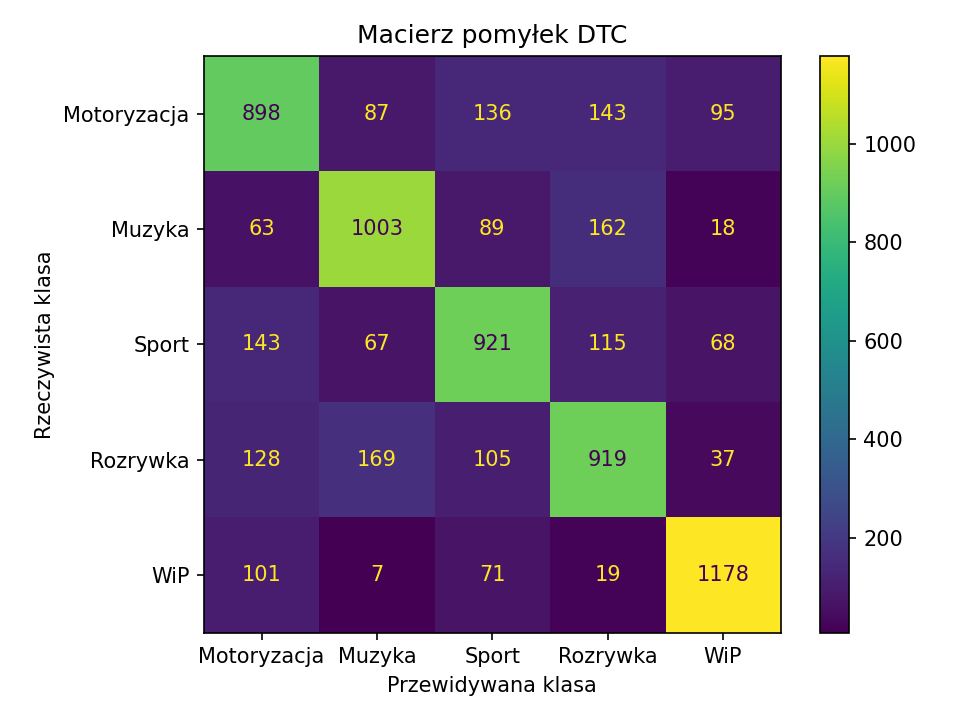
\includegraphics[width=0.5\textwidth]{Images/klasyfikacja DTC.png}
    \label{fig:DTC}
\end{figure}

\begin{figure}[H]
    \centering
    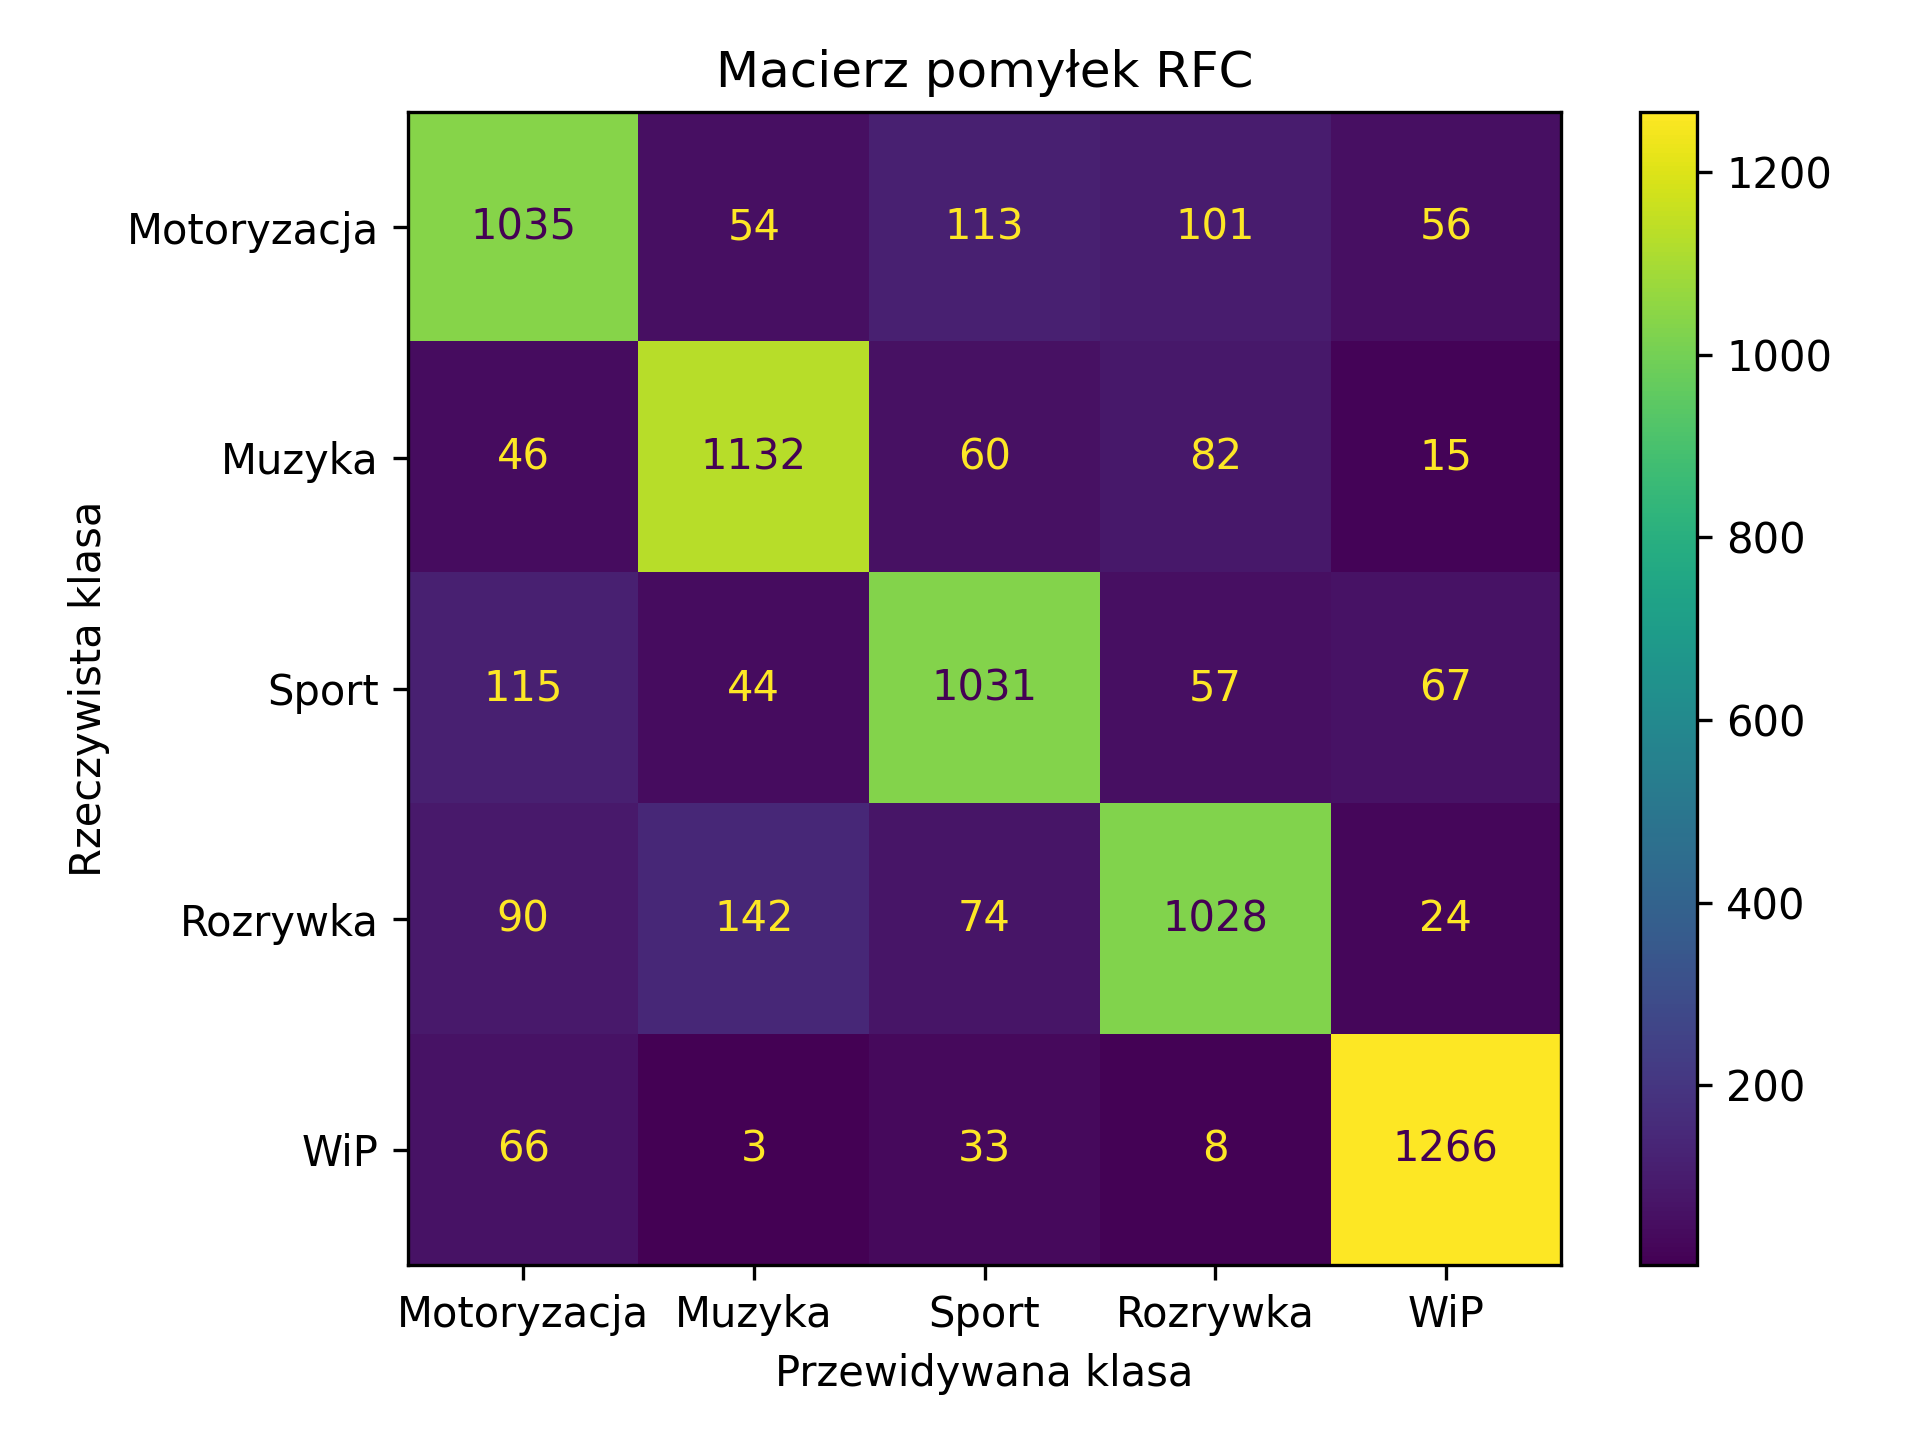
\includegraphics[width=0.5\textwidth]{Images/klasyfikacja RFC.png}
    \label{fig:RFC}
\end{figure}

Na macierzy pomyłek możemy zobaczyć dokładnie, ile razy model przewidywał jakąś kategorię, a jaka była naprawdę.

Warto sprawdzić czy, nasz model nie poradzi sobie lepiej bez jakiegoś atrybutu przy klasyfikacji:


\begin{table}[htbp]
\centering
\label{tab:results}
\rotatebox{90}{
\begin{tabular}{|l|c|c|c|c|c|c|c|}
\hline
\multirow{2}{*}{Model} & \multirow{2}{*}{Bez} & \multicolumn{6}{c|}{F1-score} \\
\cline{3-8}
& &Motoryzacja & Muzyka & Sport & Rozrywka & Wip & Dokładność \\
\hline
\multirow{6}{*}{DTC} &  Liczba Wyświetleń & 0.62 & 0.73 & 0.63 & 0.66 & 0.78 & 0.69 \\
\cline{2-8}
& Liczba komentarzy & 0.58 & 0.74 & 0.61 & 0.65 & 0.62 & 0.64 \\
\cline{2-8}
& Liczba polubień & 0.59 & 0.72 & 0.63 & 0.67 & 0.83 & 0.69\\
\cline{2-8}
& Czy dla dzieci & 0.67 & 0.73 & 0.69 & 0.67 & 0.83 & 0.72 \\
\cline{2-8}
& Czas trwania & 0.57 & 0.69 & 0.63 & 0.59 & 0.81 & 0.66 \\
\cline{2-8}
& Minuty po północy & 0.61 & 0.71 & 0.66 & 0.62 & 0.82 & 0.68 \\
\hline
\multirow{6}{*}{RFC} &  Liczba Wyświetleń & 0.73 & 0.81 & 0.72 & 0.75 & 0.85 & 0.77 \\
\cline{2-8}
& Liczba komentarzy & 0.69 & 0.8 & 0.71 & 0.75 & 0.71 & 0.73\\
\cline{2-8}
& Liczba polubień & 0.68 & 0.79 & 0.7 & 0.76 & 0.89 & 0.77 \\
\cline{2-8}
& Czy dla dzieci & 0.76 & 0.82 & 0.78 & 0.77 & 0.89 & 0.8\\
\cline{2-8}
& Czas trwania & 0.68 & 0.75 & 0.73 & 0.66 & 0.87 & 0.74 \\
\cline{2-8}
& Minuty po północy & 0.69 & 0.79 & 0.73 & 0.71 & 0.88 & 0.76\\
\hline
\end{tabular}}
\vspace{15pt}
\end{table}

\newpage
Z tabelki możemy odczytać, że każdy z argumentów polepsza naszą klasyfikację, nawet "czy dla dzieci", chociaż są to tylko 2 punkty procentowe, ale bardzo dla nas ważne.





